% !TeX TS-program = lualatex
%----------------------------------------------------------------------------------------
%    PACKAGES AND THEMES
%----------------------------------------------------------------------------------------

\documentclass[aspectratio=169,xcolor=dvipsnames]{beamer}
\usetheme{SimpleDarkBlue}

\usepackage{booktabs}  % professionally typeset tables
\usepackage{amsmath}
\usepackage{amsthm}
\usepackage{amssymb} 
\usepackage{amsfonts}
\usepackage{tikz}
\usepackage{tikz-qtree}
\usetikzlibrary{calc,positioning}
\usepackage{pgfpages}
% \setbeameroption{show notes on second screen}
\usepackage{multicol}
\usepackage{textcomp}  % better copyright sign, among other things
\usepackage{lipsum}    % filler text
\usepackage{lscape}
\usepackage{longtable}
\usepackage{siunitx}
% Please add the following required packages to your document preamble:
\usepackage{multirow}
\usepackage[table,xcdraw]{xcolor}
\usepackage{xstring}
\usepackage{relsize}
\usepackage{hyperref}
\usepackage{graphicx} % Allows including images
\usepackage{fontspec}
%\usepackage{helvet}
\setsansfont{Open Sans}
%----------------------------------------------------------------------------------------
%    TITLE PAGE
%----------------------------------------------------------------------------------------

\title{Probability Estimation Using Monte Carlo Simulation of Boolean Logic on Hardware-Accelerated Platforms}

\author{Arjun Earthperson}

\institute
{
    PhD Candidate, PRA Group\\
}
%----------------------------------------------------------------------------------------
%    PRESENTATION SLIDES
%----------------------------------------------------------------------------------------

\begin{document}
% \hypersetup{
% 	pdfkeywords={SP-Right}
% }
\begin{frame}
    % Print the title page as the first slide
    \titlepage
\end{frame}


\section*{Birds' Eye View}
\begin{frame}
  % \begin{multicols}{2}

  % \end{multicols}
    {\small{\tableofcontents}}
\end{frame}



\section{Emerging Opportunities}
\subsection{Evolving Hardware Landscape}
% \begin{frame}{}
% \end{frame}
\subsection{AI-assisted Workflows}
% \begin{frame}{}
% \end{frame}

\section{PRA Models as Probabilistic Circuits}
\subsection{Knowledge Compilation}
\subsection{Efficient Queries}

\section{Data-Parallel Monte Carlo for Probabilistic Circuits}
\subsection{Bitwise K/N Operations}


\section{Preliminary Case Study: Aralia Dataset}
\subsection{Performance \& Accuracy Benchmarks}

\section{Next Steps}
\subsection{G-PWR \& MHGTR Models}
\subsection{Importance Sampling}

\section{Upcoming Work}
\subsection{PRA Semantic Embedding Models}
\subsection{Gradient Computation for Learning}

% % \input{0_intro/1_acknowledgements}
% \input{0_intro/2_about_me}
% \input{0_intro/3_prev_work}

% \begin{frame}{Overview}
%     \tableofcontents
% \end{frame}

\section{Emerging Opportunities}
\subsection{Emerging Opportunities}

\begin{frame}[t]{Evolving Hardware Landscape}
\textbf{Industry responding to emerging ML compute challenges by investing heavily in data-parallel hardware}
  \begin{itemize} 
    \item GPUs, tensor cores provide high throughput for integer operations.
    \item Current-gen consumer hardware already supports specialized ops (Intel AMX, VNNI).
  \end{itemize}
  \vspace{8pt}
\textbf{Designed for Massive Workloads}
  \begin{itemize} 
    \item $\approx10^9$ parameters on mobile devices, $\approx10^{12}$ on HPC/cloud.
    \item Comparatively, largest PRA models: $\approx10^6$ parameters.
  \end{itemize}
\end{frame}

\begin{frame}[t]{Evolving Hardware Landscape}
\textbf{Industry responding to emerging ML compute challenges by investing heavily in data-parallel hardware}
  \begin{itemize} 
    \item GPUs, tensor cores provide high throughput for integer operations.
    \item Current-gen consumer hardware already supports specialized ops (Intel AMX, VNNI).
  \end{itemize}
  \vspace{8pt}
\textbf{Designed for Massive Workloads}
  \begin{itemize} 
    \item $\approx10^9$ parameters on mobile devices, $\approx10^{12}$ on HPC/cloud.
    \item Comparatively, largest PRA models: $\approx10^6$ parameters.
  \end{itemize}
      \vspace{12pt}
  \textit{But PRA models have no overlap with ML models.}\\
\end{frame}

\begin{frame}[t]{Evolving Hardware Landscape}
\textbf{Industry responding to emerging ML compute challenges by investing heavily in data-parallel hardware}
  \begin{itemize} 
    \item GPUs, tensor cores provide high throughput for integer operations.
    \item Current-gen consumer hardware already supports specialized ops (Intel AMX, VNNI).
  \end{itemize}
  \vspace{8pt}
\textbf{Designed for Massive Workloads}
  \begin{itemize} 
    \item $\approx10^9$ parameters on mobile devices, $\approx10^{12}$ on HPC/cloud.
    \item Comparatively, largest PRA models: $\approx10^6$ parameters.
  \end{itemize}
      \vspace{12pt}
  \textit{But PRA models have no overlap with ML models(?)}\\
\end{frame}

\begin{frame}[t]{Evolving Hardware Landscape}
\textbf{Industry responding to emerging ML compute challenges by investing heavily in data-parallel hardware}
  \begin{itemize} 
    \item GPUs, tensor cores provide high throughput for integer operations.
    \item Current-gen consumer hardware already supports specialized ops (Intel AMX, VNNI).
  \end{itemize}
  \vspace{8pt}
\textbf{Designed for Massive Workloads}
  \begin{itemize} 
    \item $\approx10^9$ parameters on mobile devices, $\approx10^{12}$ on HPC/cloud.
    \item Comparatively, largest PRA models: $\approx10^6 \text{ to } 10^9$ parameters.
  \end{itemize}
    \vspace{12pt}
\textit{But PRA models have no overlap with ML models (?)} - \textbf{Research Question}\\
\textit{Probability estimation analogous to inference in feed-forward networks.}
\end{frame}

\note{
    \begin{itemize}
        \item here, I want to say that hardware vendors, and the industry in general is responding to emerging AI/ML compute challenges by investing heavily in data-parallel hardware (GPGPU, ASIC accelerators, tensor processors). Ops/W/die is improving, opening up opportunities on HPC/cloud as well edge/personal devices. At the same time, the sheer complexity of AI/ML models is many orders of magnitude (trillions of params) larger vs PRA models (currently hundreds of thousands to millions of params). If the algorithms could leverage the appropriate hardware, PRA quantification (in terms of size) would have been solved by now. But, SOTA PRA methods are nowhere close to being able to leverage this new/emerging hardware. We need new methods.
    \end{itemize}
}
\subsection{Research Contribution}

\section{Introduction}
\subsection{Research Agenda}
\begin{frame}{Research Questions}
  \begin{itemize}
    \item{How can large-scale PRA models be quantified efficiently?}
        \vspace{4pt}
    \item {What are the overlaps between PRA models and Probabilistic Circuits?}
    \vspace{4pt}
    \item{What guarantees can be made about tractability and accuracy when using Monte Carlo for probability estimation?}
        \vspace{4pt}
    \item {What techniques can be developed to exploit native hardware parallelism for PRA quantification?}
    \vspace{4pt}

  \end{itemize}
\end{frame}

\begin{frame}[allowframebreaks]{Research Contribution}
\begin{enumerate}
\item \textbf{Bridge PRA modeling semantics with Probabilistic Circuits}
\vspace{4pt}
\item \textbf{Develop data-parallel Monte Carlo methods for evaluating Boolean circuits}
\vspace{4pt}
\item \textbf{Open-source implementations and benchmarks}
\vspace{4pt}
\item \textbf{Develop Monte Carlo sampling techniques for computing partial-derivatives on Boolean circuits}  
\end{enumerate}
\end{frame}

%\item \textbf{Data-Parallel Monte Carlo for Expectation Queries over Boolean Circuits}

% \section{Motivation}
% \subsection{PRA Unmet Needs}
\begin{frame}[t]{Long-Standing Needs in PRA Quantification}
  \begin{itemize}
    \item Large-scale PRA models ($\geq\space\approx10^4$ components) remain computationally taxing.
    \item To ease burden, approximations are used, implicating accuracy.
    \item No knobs for controlling trade-off between accuracy and speed.
  \end{itemize}
\end{frame}

\begin{frame}[t]{Long-Standing Needs in PRA Quantification}
  \begin{itemize}
    \item Large-scale PRA models ($\geq\space\approx10^4$ components) remain computationally taxing.
    \item To ease burden, approximations are used, implicating accuracy.
    \item No knobs for controlling trade-off between accuracy and speed.
  \end{itemize}
    \vspace{16pt}
    Large-scale PRA models still takes days to quantify.
\end{frame}

%% 

% % With the objective of bridging the gap between PDAG and probabilistic circuits, generate a section, including multiple frames, that (1) introduce the concept of the triplet definition of risk, (2) scenario modeling in PRA,  (3) event trees, (4) fault trees, (5) event tree / fault tree linking (together as a PRA model), (6) the concept of a PDAG, (7) PRA model as a PDAG. So, include at-least 7 frames, but you can use more. Include equations and definitions where appropriate.

\section{Research Objective 1: Bridge PRA Modeling Semantics with Probabilistic Circuits}
\begin{frame}
    \Large{\centerline{\textbf{Research Objective 1}}}
    \vspace{6pt}
    \large{\centerline{\textbf{Bridge PRA Modeling Semantics with Probabilistic Circuits}}}
\end{frame}

\subsection{PRA Overview}
\begin{frame}[allowframebreaks]
\frametitle{The Triplet Definition of Risk}
\begin{itemize}
  \item Define risk as a set of triplets, each representing:
    \begin{enumerate}
      \item What can go wrong? (\(S_i\))
      \item How likely is it to happen? (\(L_i\))
      \item What are the consequences? (\(X_i\))
    \end{enumerate}
        \vspace{6pt}
  \item
    \begin{equation}
    \label{eq:risk_triplets_slides}
      R \;=\;\bigl\{\langle S_i,\,L_i,\,X_i\rangle\bigr\}_{c},
    \end{equation}
    \(\,c\) represents completeness in enumerating \emph{all} relevant scenarios.
\end{itemize}
\end{frame}

\begin{frame}[allowframebreaks]
\frametitle{Scenario \(S_i\) Modeling in PRA}
\begin{itemize}
  \item Each scenario unfolds from initiating events (IEs), followed by conditional branching events.
          \vspace{6pt}
  \item Fundamental goal: assign probabilities to these scenarios {and} assess resulting outcomes (e.g., core damage, large release).
          \vspace{6pt}
  \item Implementation typically uses structured diagrams such as:
    \begin{itemize}
      \item Event Trees (ETs): forward chaining from IE to various end states.
      \item Fault Trees (FTs): top-down decomposition to basic events (component failures).
    \end{itemize}
\end{itemize}
\end{frame}

\begin{frame}[t, allowframebreaks]
\frametitle{Event Trees}
\begin{figure}[ht!]
\centering
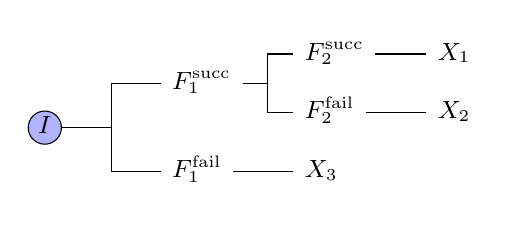
\begin{tikzpicture}
\tikzset{grow'=right,level distance=48pt}
\tikzset{execute at begin node=\strut}
\tikzset{every tree node/.style={anchor=base west}}
\tikzset{
    edge from parent/.append style={very thick},
    edge from parent/.style={
        draw,
        edge from parent path={
            (\tikzparentnode.east) -| ($(\tikzparentnode.east)!0.5!(\tikzchildnode.west)$) |- (\tikzchildnode.west)
        },
    },
    every node/.style={anchor=center,font=\small\bfseries, text centered, inner sep=0pt},
    every level 0 node/.style={circle, font=\small\bfseries, draw, fill=blue!30, inner sep=0pt},
    every internal node/.style={font=\small, inner sep=4pt},
    every leaf node/.style={rectangle, draw, fill=blue!30, minimum width=2.5cm, text centered},
    frontier/.style={distance from root=400pt},
}
\Tree [.\(I\)
    [.\(F_1^{\text{succ}}\)
        [.\(F_2^{\text{succ}}\)
            [.\(X_1\) ]
        ]
        [.\(F_2^{\text{fail}}\)
            [.\(X_2\) ]
        ]
    ]
    [.\(F_1^{\text{fail}}\)
        [.\(X_3\) ]
    ]
]
\end{tikzpicture}
\caption{Illustrative event tree with an initiating event \(I\), two functional events \(F_1\) and \(F_2\), and three end-states \(X_1, X_2, X_3\).}
\label{fig:event_tree_example}
\end{figure}
\begin{itemize}
  \item An Event Tree represents how an initiating event \(I\) can branch into multiple functional-event outcomes.
  \item Each functional event \(F_k\) may succeed or fail, driving the path toward a distinct end-state \(X_j\).  
  \item If \(\omega_j\) denotes one branch leading to \(X_j\), then the branch probability often factors as 
    \[
      p(\omega_j) \;=\; p(I)\;\times\;\prod_{k=1}^{n} \; p\bigl(F_k^{\alpha_k} \;\mid\; \text{all previous outcomes}\bigr).
    \]
  \item As a logical expression, each \(\omega_j\) translates to an AND of success/failure literals, and the overall set of end-states is an OR of these branches:
    \[
      \Omega \;=\;\omega_1 \;\lor\;\omega_2 \;\lor\;\dots\;\lor\;\omega_m.
    \]
  \item Consequently, ETs are in \emph{sum of products} (SOP) or \emph{disjunctive normal form} (DNF), where each product term identifies one success/failure path and the scenario-level outcome is the logical OR across all such paths.
  \vspace{4pt}
  \item Graphically straightforward, but can combinatorially expand for deep branching.
\end{itemize}
\end{frame}

\begin{frame}[t, allowframebreaks]
\frametitle{Fault Trees}
    \begin{figure}[h]
    \centering
    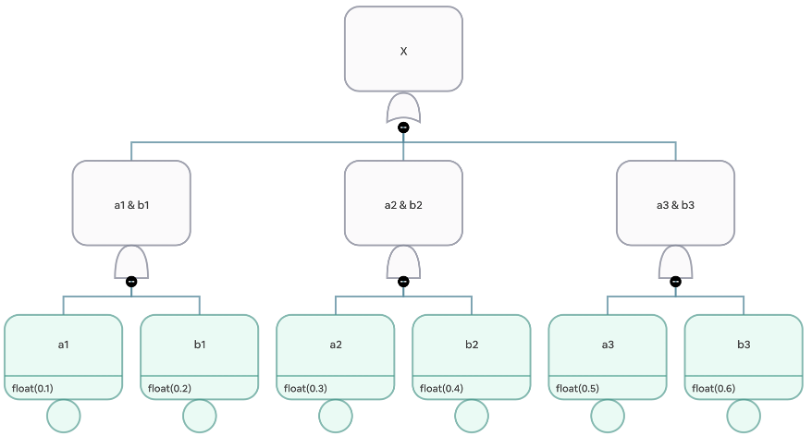
\includegraphics[width=0.5\textwidth]{1_concepts/ft.png}
    \caption{Fault tree with 6 basic events, top event $X = (a_1\bigwedge b_1) \bigvee (a_2\bigwedge b_2) \bigvee (a_3\bigwedge b_3)$}
    \label{fig:ft}
\end{figure}
\begin{itemize}
  \item A Fault Tree describes how a top event (system failure) can result from lower-level component or subsystem failures.
  \item Internal gates (AND, OR, \(k\)-of-\(n\), etc.) combine events in logical fashion:
    \[
      \text{Output} \;=\;
      \begin{cases}
         \bigwedge_{i=1}^k e_i, & \text{(AND)}\\
         \bigvee_{i=1}^k e_i, & \text{(OR)}\\
         \dots
      \end{cases}
    \]
  \item Basic events (BEs) in the leaves have assigned probabilities \(p(b)\).  Independence often assumed unless modeling common-cause failures.
  \item The top event failure probability can be written as:
    \begin{equation}
    \label{eq:top_event_probability_slides}
    \Pr[\text{Top Fail}] \;=\; \sum_{S \subseteq \,\mathcal{B}} 
      \Bigl[
        \pi_{F}(S, \text{Top}) 
        \prod_{b\in S} p(b)\prod_{b\notin S}[1 - p(b)]
      \Bigr].
    \end{equation}
\end{itemize}
\end{frame}

\begin{frame}[t, allowframebreaks]
\frametitle{Linking Event Trees and Fault Trees in PRA}
\begin{itemize}
  \item Real systems often combine:
    \begin{itemize}
      \item Forward branching dynamics via Event Trees (ET).
      \item Subsystem or component reliability logic via Fault Trees (FT).
    \end{itemize}
  \item An event tree branch may call a specific FT top event to collect system failure or success.
  \item Conversely, a fault tree output may feed back into an event tree branch as an initiating event or functional node outcome.
  \item This multi-level interconnection \(\implies\) a need for a unified model capturing both forward branching (ET) and hierarchical failure logic (FT).
\end{itemize}
\end{frame}

\begin{frame}[t, allowframebreaks]
\frametitle{Probabilistic Directed Acyclic Graph (PDAG)}
\begin{itemize}
  \item A PDAG is a Directed Acyclic Graph whose edges carry either:
    \begin{itemize}
      \item Conditional probabilities (e.g., for event tree branches).  
      \item Logical dependencies (e.g., for fault tree gates).
    \end{itemize}
  \item Nodes may include:
    \begin{itemize}
      \item Basic events (BEs) with known probabilities.
      \item ET or FT intermediate events storing partial results.
      \item Any top-level node (e.g., a final end-state) with no children.
    \end{itemize}
  \item The absence of cycles guarantees consistent flow from initial seeds (basic events, initiating events) to final outcomes.
  \item PDAG forms the structural backbone for bridging scenario-based expansions with gate-based logic in a single coherent representation.
\end{itemize}
\end{frame}

\subsection{Probabilistic Circuits Overview}
\begin{frame}[t, allowframebreaks]
\frametitle{Probabilistic Circuits: A Brief Overview}
    \begin{figure}[h]
    \centering
    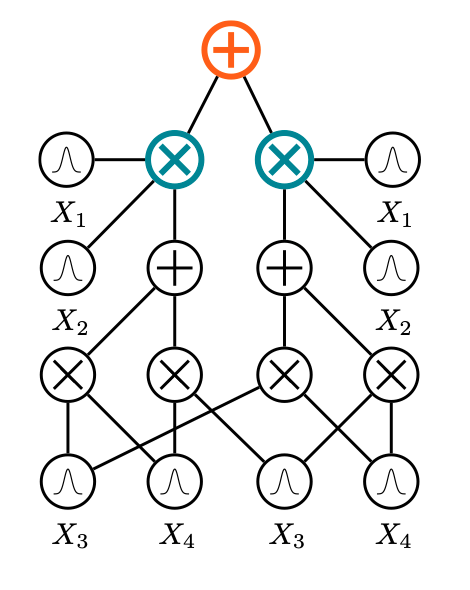
\includegraphics[height=0.5\textheight]{1_concepts/pc.png}
    \caption{Probabilistic circuit with 4 inputs $X_i$, product gates (blue), sum gate (orange)}
    \label{fig:pc}
\end{figure}
\end{frame}

\begin{frame}[t, allowframebreaks]
\begin{itemize}
  \item A \textbf{probabilistic circuit} is a directed acyclic graph (DAG) that encodes a joint probability distribution through \emph{sum-gates} and \emph{product-gates}.
  \item \textbf{Sum-gates} approximate mixture distributions:
    \[
      p_v(\mathbf{x})
      \;=\;
      \sum_{u\in \operatorname{ch}(v)} \theta_{v,u}\,p_u(\mathbf{x}),
      \quad
      \text{with }
      \sum_{u\in \operatorname{ch}(v)} \theta_{v,u} = 1.
    \]
    Each child distribution is weighted by a nonnegative parameter \(\theta_{v,u}\).
  \item \textbf{Product-gates} factorize independent variable sets:
    \[
      p_v(\mathbf{x})
      \;=\;
      \prod_{u\in \operatorname{ch}(v)} p_u\bigl(\mathbf{x}_{u}\bigr),
    \]
    assuming disjoint subsets of variables for each child \(u\).
  \item \textbf{Leaf nodes} (inputs) often correspond to known base distributions. When evaluated upward through the DAG, each internal node yields its own distribution, culminating in a root node that represents the full model.
  \item \textbf{Key motivation}:
    \begin{itemize}
      \item Tractable inference: evaluation and certain marginal or conditional queries can be performed in time proportional to circuit size.  
      \item Decomposability and modularity: separate, interpretable substructures that can be reused or combined for large-scale systems.
    \end{itemize}
\end{itemize}
\end{frame}

\subsection{PRA PDAGs to Probabilistic Circuits}
\begin{frame}[allowframebreaks]
\frametitle{Compiled PRA Graphs are PDAGs}
\begin{itemize}
  \item A unified PRA model can be viewed as
    \[
      \mathcal{M} 
      \;=\;
      \langle 
        \mathcal{V},\,\mathcal{A},\, \{p(b)\},\, \{\theta_{u\to v}\},\,\pi_{F}
      \rangle,
    \]
    where \(\mathcal{V}\) includes basic events, ET nodes, and FT gates, and \(\mathcal{A}\) is the acyclic edge set.
  \item Event-tree edges carry transitional probabilities \(\theta_{u\to v}\) summing to 1 from each node.
  \item Fault-tree nodes embed Boolean logic \(\pi_F\) that checks if inputs fail under a subset of basic events.
  \framebreak
  \item This PDAG perspective:
    \begin{itemize}
      \item Ensures systematic accounting of all scenario paths and subsystem logic.
      \item Aligns naturally with tractable Probabilistic Circuits, since each node’s distribution/function can be embedded in a sum-product style DAG.
      \item Offers a foundation for efficient Monte Carlo or advanced inference methods.
    \end{itemize}
    \vspace{6pt}
    \item Ongoing work to bridge PRA PDAG semantics with Probabilistic Circuits:
    \begin{itemize}
      \item PDAGs can be transformed to equivalent canonical forms (there are tradeoffs).
    \end{itemize}
\end{itemize}
\end{frame}
% 

\section{Research Objective 2: Develop data-parallel Monte Carlo methods for evaluating Boolean circuits}
\begin{frame}
    \Large{\centerline{\textbf{Research Objective 2}}}
    \vspace{6pt}
    \large{\centerline{\textbf{Develop data-parallel Monte Carlo methods for evaluating Boolean circuits}}}
\end{frame}

\subsection{Building a Monte Carlo Estimator for Event Probabilities}
\begin{frame}[t, allowframebreaks]
\frametitle{Boolean Functions: Basic Concepts}
\begin{itemize}
  \item Let \(\mathbf{x} = (x_1, x_2, \dots, x_n)\) be a vector of \(n\) Boolean variables, each \(x_i \in \{0,1\}\).
  \item A \emph{Boolean function} is any map \(F(\mathbf{x}): \{0,1\}^n \to \{0,1\}\).
  \item Example: If \(F\) encodes “system fails,” then \(F(\mathbf{x}) = 1\) signifies a failure mode, where \(\mathbf{x}\) captures component states.
  \item Modeling perspective:
    \begin{itemize}
      \item AND, OR, NOT, \(k\)-of-\(n\) gates allow composing complex logic.  
      \item Each \(F\) can be evaluated deterministically if we know \(\mathbf{x}\).
    \end{itemize}
\end{itemize}
\end{frame}

\begin{frame}[t, allowframebreaks]
\frametitle{Exact Probability Estimation: Inclusion-Exclusion}
\begin{itemize}
  \item Suppose each \(x_i\) has a probability \(p_i = \Pr[x_i=1]\), assuming independence.
  \item We want \(\Pr[F(\mathbf{x}) = 1]\), which is
  \[
    \Pr\bigl[F(\mathbf{X})=1\bigr]
    \;=\; 
    \sum_{\mathbf{x}\in \{0,1\}^n}
      F(\mathbf{x}) 
      \prod_{i=1}^n
      \bigl[p_i^{\,x_i}(1-p_i)^{\,1-x_i}\bigr].
  \]
  \item For sets of events, using the \emph{inclusion-exclusion principle}:
  \[
    \Pr\Bigl(\bigcup_{i=1}^n E_i\Bigr)
    \;=\;
    \sum_{k=1}^n \;(-1)^{k+1} 
    \;\;\sum_{1\le i_1< \cdots < i_k\le n}
    \!\Pr\bigl(E_{i_1}\cap\dots\cap E_{i_k}\bigr).
  \]

\end{itemize}
\end{frame}

\begin{frame}[allowframebreaks]
\frametitle{Approximation Methods: REA and MCUB}
 For large \(n\), exact enumeration of subsets is exponential, making it impractical for large Boolean circuits.
 \vspace{8pt}
\begin{itemize}
  \item \textbf{Rare-Event Approximation (REA):}
    \begin{itemize}
      \item Assumes each event has small probability \(p_i \ll 1\).
      \item Overlaps (intersections of multiple failures) are deemed negligible.
      \item Probability of the union \(\approx \sum_{i} \Pr[E_i]\), ignoring higher-order terms.
    \end{itemize}
\framebreak
  \item \textbf{Min-Cut Upper Bound (MCUB):}
    \begin{equation}
    \label{eq:mcub_slides}
      \Pr\Bigl[\bigcup_{C \in \{\mathrm{MCS}\}} C\Bigr]
      \;\le\;
      \sum_{C \in \{\mathrm{MCS}\}}
      \;\prod_{b \in C} p_b ,
    \end{equation}
    \begin{itemize}
      \item Interprets each minimal cut set (MCS) as a distinct mechanism for failure.
      \item Sums (over)estimate total failure if MCSs share components.
      \item Often used as a conservative bound in safety analyses.
    \end{itemize}
  \vspace{6pt}
  \item Both methods reduce complexity but can misestimate the true probability when events are not truly rare or heavily intersect.
\end{itemize}
\end{frame}

\begin{frame}[t, allowframebreaks]
\frametitle{Monte Carlo Sampling}
\begin{itemize}
  \item Rather than summing or bounding all combinations of failures, \emph{simulate} random draws of \(\mathbf{X}\).
  \item Each Monte Carlo iteration:
    \begin{enumerate}
      \item Sample \(x_1, x_2,\dots,x_n \overset{\text{i.i.d.}}{\sim} \prod p(x_i)\).
      \item Evaluate the Boolean function \(F(\mathbf{x})\) (cost is just logical gate evaluation).
      \item Collect whether \(F(\mathbf{x})=1\) (failure) or 0 (success).
    \end{enumerate}
  \item Repeating for many samples \(\{\mathbf{x}^{(1)}, \dots, \mathbf{x}^{(N)}\}\) yields a \emph{sample average} estimate of the probability.
  \item Benefits:
    \begin{itemize}
      \item Bypasses explicit inclusion-exclusion expansions.
      \item Straightforward to parallelize (evaluate each draw in separate threads or blocks).
    \end{itemize}
\end{itemize}
\end{frame}

\begin{frame}[t, allowframebreaks]
\frametitle{Estimator for the Expected Value (i.e., Probability)}
\begin{itemize}
  \item A Boolean function \(F(\mathbf{x})\) can be viewed as an indicator function: \(F(\mathbf{x}) \in \{0,1\}\).
  \item The event \(\{F(\mathbf{X})=1\}\) has probability \(\mathbb{E}[F(\mathbf{X})]\).
  \item \textbf{Monte Carlo estimator:}
    \[
      \widehat{P}_N
      \;=\;
      \frac{1}{N}\sum_{i=1}^N 
      F\!\bigl(\mathbf{x}^{(i)}\bigr),
    \]
    where each \(\mathbf{x}^{(i)}\) is a random draw from the input distribution.
  \item By the Law of Large Numbers,
    \[
      \lim_{N \to \infty}\;\widehat{P}_N
      \;=\;
      \Pr\bigl[F(\mathbf{X})=1\bigr],
      \quad \text{almost surely}.
    \]
  \item Error decreases at rate \(\mathcal{O}(1/\sqrt{N})\), analyzed via the Central Limit Theorem.
\end{itemize}
\end{frame}

\begin{frame}[t]
\frametitle{Boolean Derivatives: Definition and Interpretation}
\begin{itemize}
\item \textbf{Boolean Derivative Concept:}  
  For a Boolean function \(F(\mathbf{x})\) with \(\mathbf{x}=(x_1,\ldots,x_n)\), the derivative with respect to \(x_i\) is defined via XOR:
  \[
    \frac{\partial F}{\partial x_i}
    \;=\;
    F(x_i=0,\mathbf{x}_{-i})
    \;\oplus\;
    F(x_i=1,\mathbf{x}_{-i}),
  \]
  where \(\oplus\) denotes the exclusive-OR operation, and \(\mathbf{x}_{-i}\) are all variables except \(x_i\).
\item \textbf{Interpretation:}  
  \begin{itemize}
    \item \(\frac{\partial F}{\partial x_i}(\mathbf{x})=1\) whenever \emph{flipping} \(x_i\) changes the value of \(F\) under the specific configuration \(\mathbf{x}_{-i}\).  
    \item Captures \emph{sensitivity}: if \(\frac{\partial F}{\partial x_i}\) rarely equals \(1\), then \(F\) is robust to changes in \(x_i\).  
  \end{itemize}
\end{itemize}
\end{frame}

\begin{frame}[allowframebreaks]
\frametitle{Extension to Monte Carlo Estimation of Boolean Derivatives}
\begin{itemize}
  \item \textbf{Key Idea:} Estimate \(\mathbb{E}[\,\partial F / \partial x_i\,]\) by sampling random configurations \(\mathbf{x}^{(s)}\) of the Boolean inputs, then checking how \(F\) changes when \(x_i\) is flipped.
  \vspace{8pt}
  \item \textbf{Sampling Procedure:}
    \begin{enumerate}
      \item Draw \(\mathbf{x}^{(s)} = \bigl(x_1^{(s)},\dots,x_n^{(s)}\bigr)\) from the distribution of interest.  
      \item Form \(\mathbf{x}^{(s)} \oplus \mathbf{e}_i\) by flipping the \(i\)th coordinate.
      \item Compute:
        \[
          \frac{\partial F}{\partial x_i}\bigl(\mathbf{x}^{(s)}\bigr)
          \;=\;
          F\!\bigl(\mathbf{x}^{(s)}\bigr)
          \;\oplus\;
          F\!\bigl(\mathbf{x}^{(s)} \oplus \mathbf{e}_i\bigr).
        \]
    \end{enumerate}
  \item \textbf{Insight:}  
    \begin{itemize}
    \item{Sensitivity and importance analysis using sampling methods.}
    \item{Gradient computation opens a path towards learning-based tasks.}
    \end{itemize}
\end{itemize}
\end{frame}

\begin{frame}[t, allowframebreaks]
\frametitle{Avoiding Inclusion-Exclusion via Monte Carlo}
\begin{itemize}
  \item Exact expansions for large circuits require enumerating all subsets of failing components or gates, which is computationally huge.
  \item In contrast, \emph{Monte Carlo} draws a sample \(\mathbf{x}\in \{0,1\}^n\) and directly evaluates \(F(\mathbf{x})\) without enumerating \emph{all} subsets.
  \item Each run picks a single draw of failed components from the distribution. After many runs, the frequency of \(F=1\) approximates its probability.
  \item Results:
    \begin{itemize}
      \item No exponential blow-up in the number of terms.
      \item Straightforward extension to complex gate structures, correlated variables.
      \item Parallelizable on modern CPU/GPU architectures.
    \end{itemize}
\end{itemize}
\end{frame}

\begin{frame}[t, allowframebreaks]
\frametitle{Data-Parallel Implementation using SYCL}
\item \textbf{Data-Parallel Monte Carlo for Boolean Circuits:}
  \begin{itemize}
    \item{Simultaneous evaluation of \emph{all} intermediate gates, success, and failure paths.}
    \item{Relax coherence constraints - arbitrary shapes with NOT gates permitted.}
    \item{Vectorized bitwise hardware ops for logical primitives (AND, OR, XOR, etc.)}
    \item{Specialized treatment of \(k/n\) logic, without expansion.}
    \item{Simultaneous use of all available compute - GPUs, multicore CPUs.}
    \vspace{16pt}
  \end{itemize}
\end{frame}
% \section{Preliminary Case Study}
\subsection{Setup}
\begin{frame}
    \Huge{\centerline{\textbf{Preliminary Case Study}}}
\end{frame}

\subsection{Aralia Fault Tree Data Set}
\begin{frame}[t]
\frametitle{Overview: Aralia Dataset}
\begin{itemize}
  \item \textbf{Dataset Composition:} The Aralia collection consists of 43 distinct fault trees, each with varying numbers of basic events (BEs), gate types (AND, OR, K/N, XOR), and minimal cut-set counts.  
  \item \textbf{Diverse Problem Sizes:} Small trees (e.g.\ 25--32 BEs) through large models with over 1{,}500 BEs.  
  \item \textbf{Wide Probability Range:} Top-event probabilities spanning from rare events near \(10^{-13}\) to fairly likely failures with probability above 0.7.  
  \item \textbf{Model Variability:} Some trees are primarily AND/OR, others incorporate more advanced gates (K/N, XOR, NOT), providing thorough coverage of typical (and atypical) fault tree logic structures.
\end{itemize}
\end{frame}

\begin{frame}[allowframebreaks]
    

% Please add the following required packages to your document preamble:
% \usepackage{booktabs}
% \usepackage{multirow}
% \usepackage[table,xcdraw]{xcolor}
% Beamer presentation requires \usepackage{colortbl} instead of \usepackage[table,xcdraw]{xcolor}
% \usepackage{longtable}
% Note: It may be necessary to compile the document several times to get a multi-page table to line up properly
\tiny
\begin{longtable}{@{}llrrrrrrrc@{}}
\label{tab:my-table}\\
\toprule
            &          & \multicolumn{1}{c}{} & \multicolumn{5}{c}{\textbf{Logic Gates}} & \multicolumn{1}{c}{} &             \\* \cmidrule(lr){4-8}
\multirow{-2}{*}{\textbf{\#}} &
  \multirow{-2}{*}{\textbf{\begin{tabular}[c]{@{}l@{}}Fault\\ Tree\end{tabular}}} &
  \multicolumn{1}{c}{\multirow{-2}{*}{\textbf{\begin{tabular}[c]{@{}c@{}}Basic\\ Events\end{tabular}}}} &
  \multicolumn{1}{c}{\textbf{Total}} &
  \multicolumn{1}{c}{AND} &
  \multicolumn{1}{c}{K/N} &
  \multicolumn{1}{c}{XOR} &
  \multicolumn{1}{c}{NOT} &
  \multicolumn{1}{c}{\multirow{-2}{*}{\textbf{\begin{tabular}[c]{@{}c@{}}Minimal\\ Cut Sets\end{tabular}}}} &
  \multirow{-2}{*}{\textbf{\begin{tabular}[c]{@{}c@{}}Top Event\\ Probability\end{tabular}}} \\* \midrule
\endhead
%
\bottomrule
\endfoot
%
\endlastfoot
%
\textbf{1}  & baobab1  & 61                   & 84       & 16      & 9    & -    & -     & 46,188               & 1.01708E-04 \\
\textbf{2}  & baobab2  & 32                   & 40       & 5       & 6    & -    & -     & 4,805                & 7.13018E-04 \\
\textbf{3}  & baobab3  & 80                   & 107      & 46      & -    & -    & -     & 24,386               & 2.24117E-03 \\
\textbf{4}  & cea9601  & 186                  & 201      & 69      & 8    & -    & 30    & 130,281,976          & 1.48409E-03 \\
\textbf{5}  & chinese  & 25                   & 36       & 13      & -    & -    & -     & 392                  & 1.17058E-03 \\
\textbf{6}  & das9201  & 122                  & 82       & 19      & -    & -    & -     & 14,217               & 1.34237E-02 \\
\textbf{7}  & das9202  & 49                   & 36       & 10      & -    & -    & -     & 27,778               & 1.01154E-02 \\
\textbf{8}  & das9203  & 51                   & 30       & 1       & -    & -    & -     & 16,200               & 1.34880E-03 \\
\textbf{9}  & das9204  & 53                   & 30       & 12      & -    & -    & -     & 16,704               & 6.07651E-08 \\
\textbf{10} & das9205  & 51                   & 20       & 2       & -    & -    & -     & 17,280               & 1.38408E-08 \\
\textbf{11} & das9206  & 121                  & 112      & 21      & -    & -    & -     & 19,518               & 2.29687E-01 \\
\textbf{12} & das9207  & 276                  & 324      & 59      & -    & -    & -     & 25,988               & 3.46696E-01 \\
\textbf{13} & das9208  & 103                  & 145      & 33      & -    & -    & -     & 8,060                & 1.30179E-02 \\
\textbf{14} & das9209  & 109                  & 73       & 18      & -    & -    & -     & 8.20E+10             & 1.05800E-13 \\
\textbf{15} & das9601  & 122                  & 288      & 60      & 36   & 12   & 14    & 4,259                & 4.23440E-03 \\
\textbf{16} & das9701  & 267                  & 2,226    & 1,739   & -    & -    & 992   & 26,299,506           & 7.44694E-02 \\
\textbf{17} & edf9201  & 183                  & 132      & 12      & -    & -    & -     & 579,720              & 3.24591E-01 \\
\textbf{18} & edf9202  & 458                  & 435      & 45      & -    & -    & -     & 130,112              & 7.81302E-01 \\
\textbf{19} & edf9203  & 362                  & 475      & 117     & -    & -    & -     & 20,807,446           & 5.99589E-01 \\
\textbf{20} & edf9204  & 323                  & 375      & 106     & -    & -    & -     & 32,580,630           & 5.25374E-01 \\
\textbf{21} & edf9205  & 165                  & 142      & 30      & -    & -    & -     & 21,308               & 2.09351E-01 \\
\textbf{22} & edf9206  & 240                  & 362      & 126     & -    & -    & -     & 385,825,320          & 8.61500E-12 \\
\textbf{23} & edfpa14b & 311                  & 290      & 70      & -    & -    & -     & 105,955,422          & 2.95620E-01 \\
\textbf{24} & edfpa14o & 311                  & 173      & 42      & -    & -    & -     & 105,927,244          & 2.97057E-01 \\
\textbf{25} & edfpa14p & 124                  & 101      & 42      & -    & -    & -     & 415,500              & 8.07059E-02 \\
\textbf{26} & edfpa14q & 311                  & 194      & 55      & -    & -    & -     & 105,950,670          & 2.95905E-01 \\
\textbf{27} & edfpa14r & 106                  & 132      & 55      & -    & -    & -     & 380,412              & 2.09977E-02 \\
\textbf{28} & edfpa15b & 283                  & 249      & 61      & -    & -    & -     & 2,910,473            & 3.62737E-01 \\
\textbf{29} & edfpa15o & 283                  & 138      & 33      & -    & -    & -     & 2,906,753            & 3.62956E-01 \\
\textbf{30} & edfpa15p & 276                  & 324      & 33      & -    & -    & -     & 27,870               & 7.36302E-02 \\
\textbf{31} & edfpa15q & 283                  & 158      & 45      & -    & -    & -     & 2,910,473            & 3.62737E-01 \\
\textbf{32} & edfpa15r & 88                   & 110      & 45      & -    & -    & -     & 26,549               & 1.89750E-02 \\
\textbf{33} & elf9601  & 145                  & 242      & 97      & -    & -    & -     & 151,348              & 9.66291E-02 \\
\textbf{34} & ftr10    & 175                  & 94       & 26      & -    & -    & -     & 305                  & 4.48677E-01 \\
\textbf{35} & isp9601  & 143                  & 104      & 25      & 1    & -    & -     & 276,785              & 5.71245E-02 \\
\textbf{36} & isp9602  & 116                  & 122      & 26      & -    & -    & -     & 5,197,647            & 1.72447E-02 \\
\textbf{37} & isp9603  & 91                   & 95       & 37      & -    & -    & -     & 3,434                & 3.23326E-03 \\
\textbf{38} & isp9604  & 215                  & 132      & 38      & -    & -    & -     & 746,574              & 1.42751E-01 \\
\textbf{39} & isp9605  & 32                   & 40       & 8       & 6    & -    & -     & 5,630                & 1.37171E-05 \\
\textbf{40} & isp9606  & 89                   & 41       & 14      & -    & -    & -     & 1,776                & 5.43174E-02 \\
\textbf{41} & isp9607  & 74                   & 65       & 23      & -    & -    & -     & 150,436              & 9.49510E-07 \\
\textbf{42} & jbd9601  & 533                  & 315      & 71      & -    & -    & -     & 150,436              & 7.55091E-01 \\
\rowcolor[HTML]{F2F2F2} 
\textbf{43} & nus9601  & 1,567                & 1,622    & 392     & 47   & -    & -     & unknown              & unknown     \\* \bottomrule
\end{longtable}
\end{frame}

\subsection{Benchmarking Procedure}
\begin{frame}[t]
\frametitle{Benchmarking Setup: Hardware and Environment}
\begin{itemize}
  \item \textbf{Target Hardware:}
    \begin{itemize}
      \item GPU: NVIDIA\textsuperscript{\textregistered} GeForce GTX 1660 SUPER (6\,GB GDDR6, 1{,}408 CUDA cores).
      \item CPU: Intel\textsuperscript{\textregistered} Core\textsuperscript{TM} i7-10700 (2.90\,GHz, turbo-boost, hyperthreading).
    \end{itemize}
  \item \textbf{Software Stack:}
    \begin{itemize}
      \item SYCL-based (AdaptiveCpp/HipSYCL), with LLVM-IR JIT for kernel compilation.
      \item Compiler optimization at \texttt{-O3} for efficient code generation.
      \item Repeated runs (5+) to mitigate transient variations.
    \end{itemize}
  \item \textbf{Measured Time:} Includes entire wall-clock duration, from host-device transfers and JIT compilation to final result collection.
\end{itemize}
\end{frame}

\begin{frame}[t]
\frametitle{Monte Carlo Execution and Implementation}
\begin{itemize}
  \item \textbf{Sampling Strategy:}
    \begin{itemize}
      \item Single pass per fault tree, generating as many samples as fit in 6\,GB GPU memory.  
      \item 128-bit Philox4x32x10 pseudo-random number generator, parallel threads.
    \end{itemize}
  \item \textbf{Bit-Packing Optimization:}
    \begin{itemize}
      \item Each group of 64 Monte Carlo outcomes stored in a single 64-bit word.  
      \item Enables vectorized instructions (e.g.\ \texttt{popcount}) and reduces memory I/O.
    \end{itemize}
  \item \textbf{Data Types:}
    \begin{itemize}
      \item Tallies in 64-bit integers.  
      \item Probability accumulations in double precision (64-bit float).  
    \end{itemize}
\end{itemize}
\end{frame}

\begin{frame}[allowframebreaks]
    \begin{figure}[h]
    \centering
    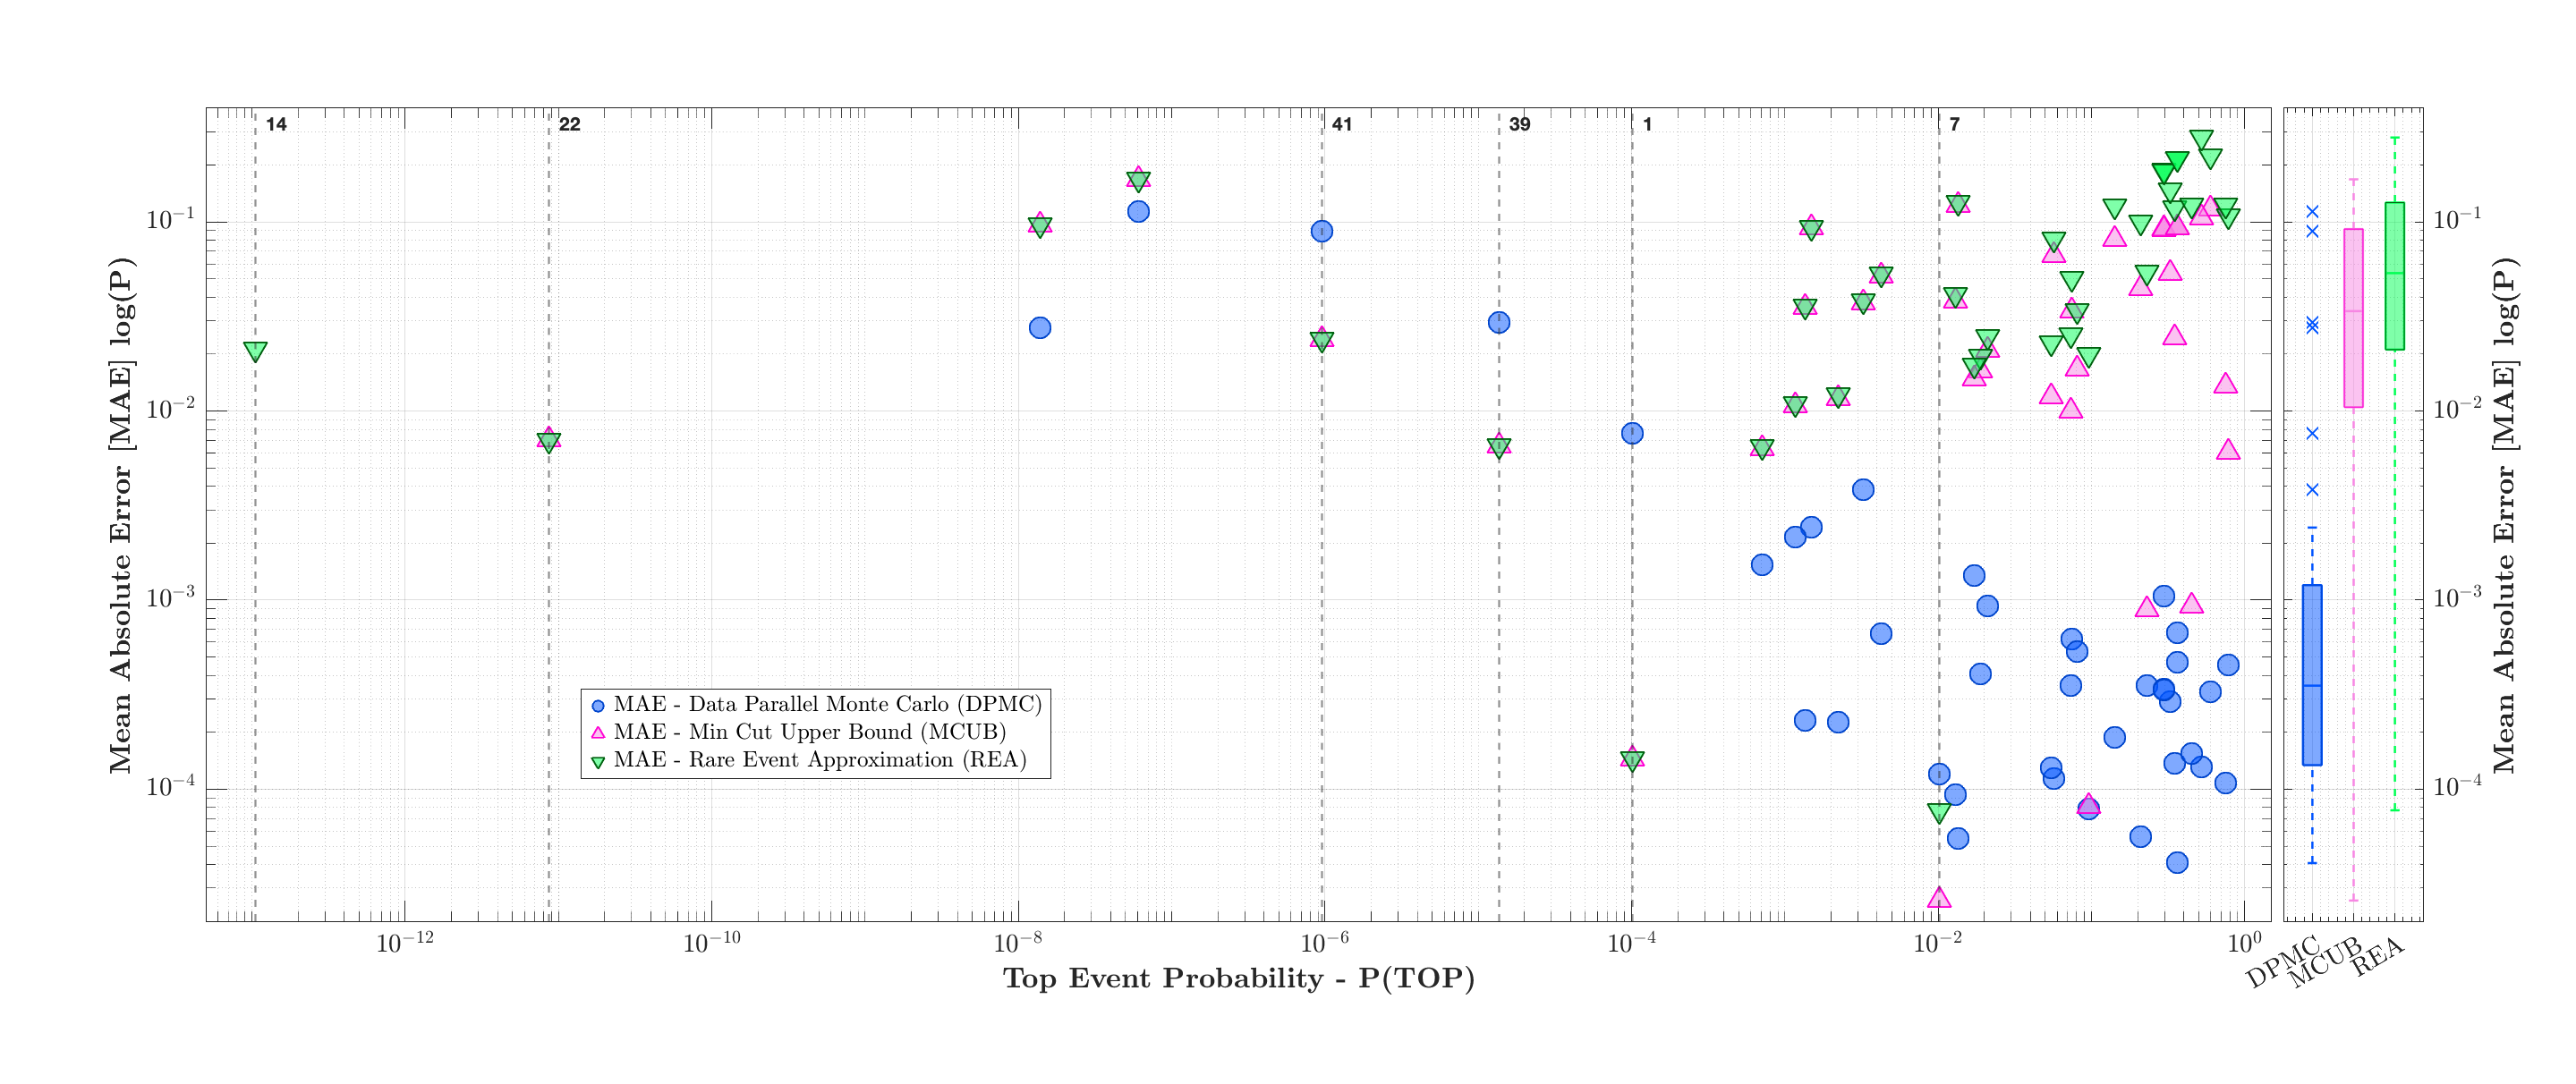
\includegraphics[width=0.9\textwidth]{4_casestudy/error_vs_prob_detailed.png}
    \caption{Mean Absolute Error – Exact (BDD) vs Approximate Methods}
    \label{fig:mae_vs_logp}
\end{figure}
\end{frame}

\begin{frame}[allowframebreaks]
    \begin{figure}[h]
    \centering
    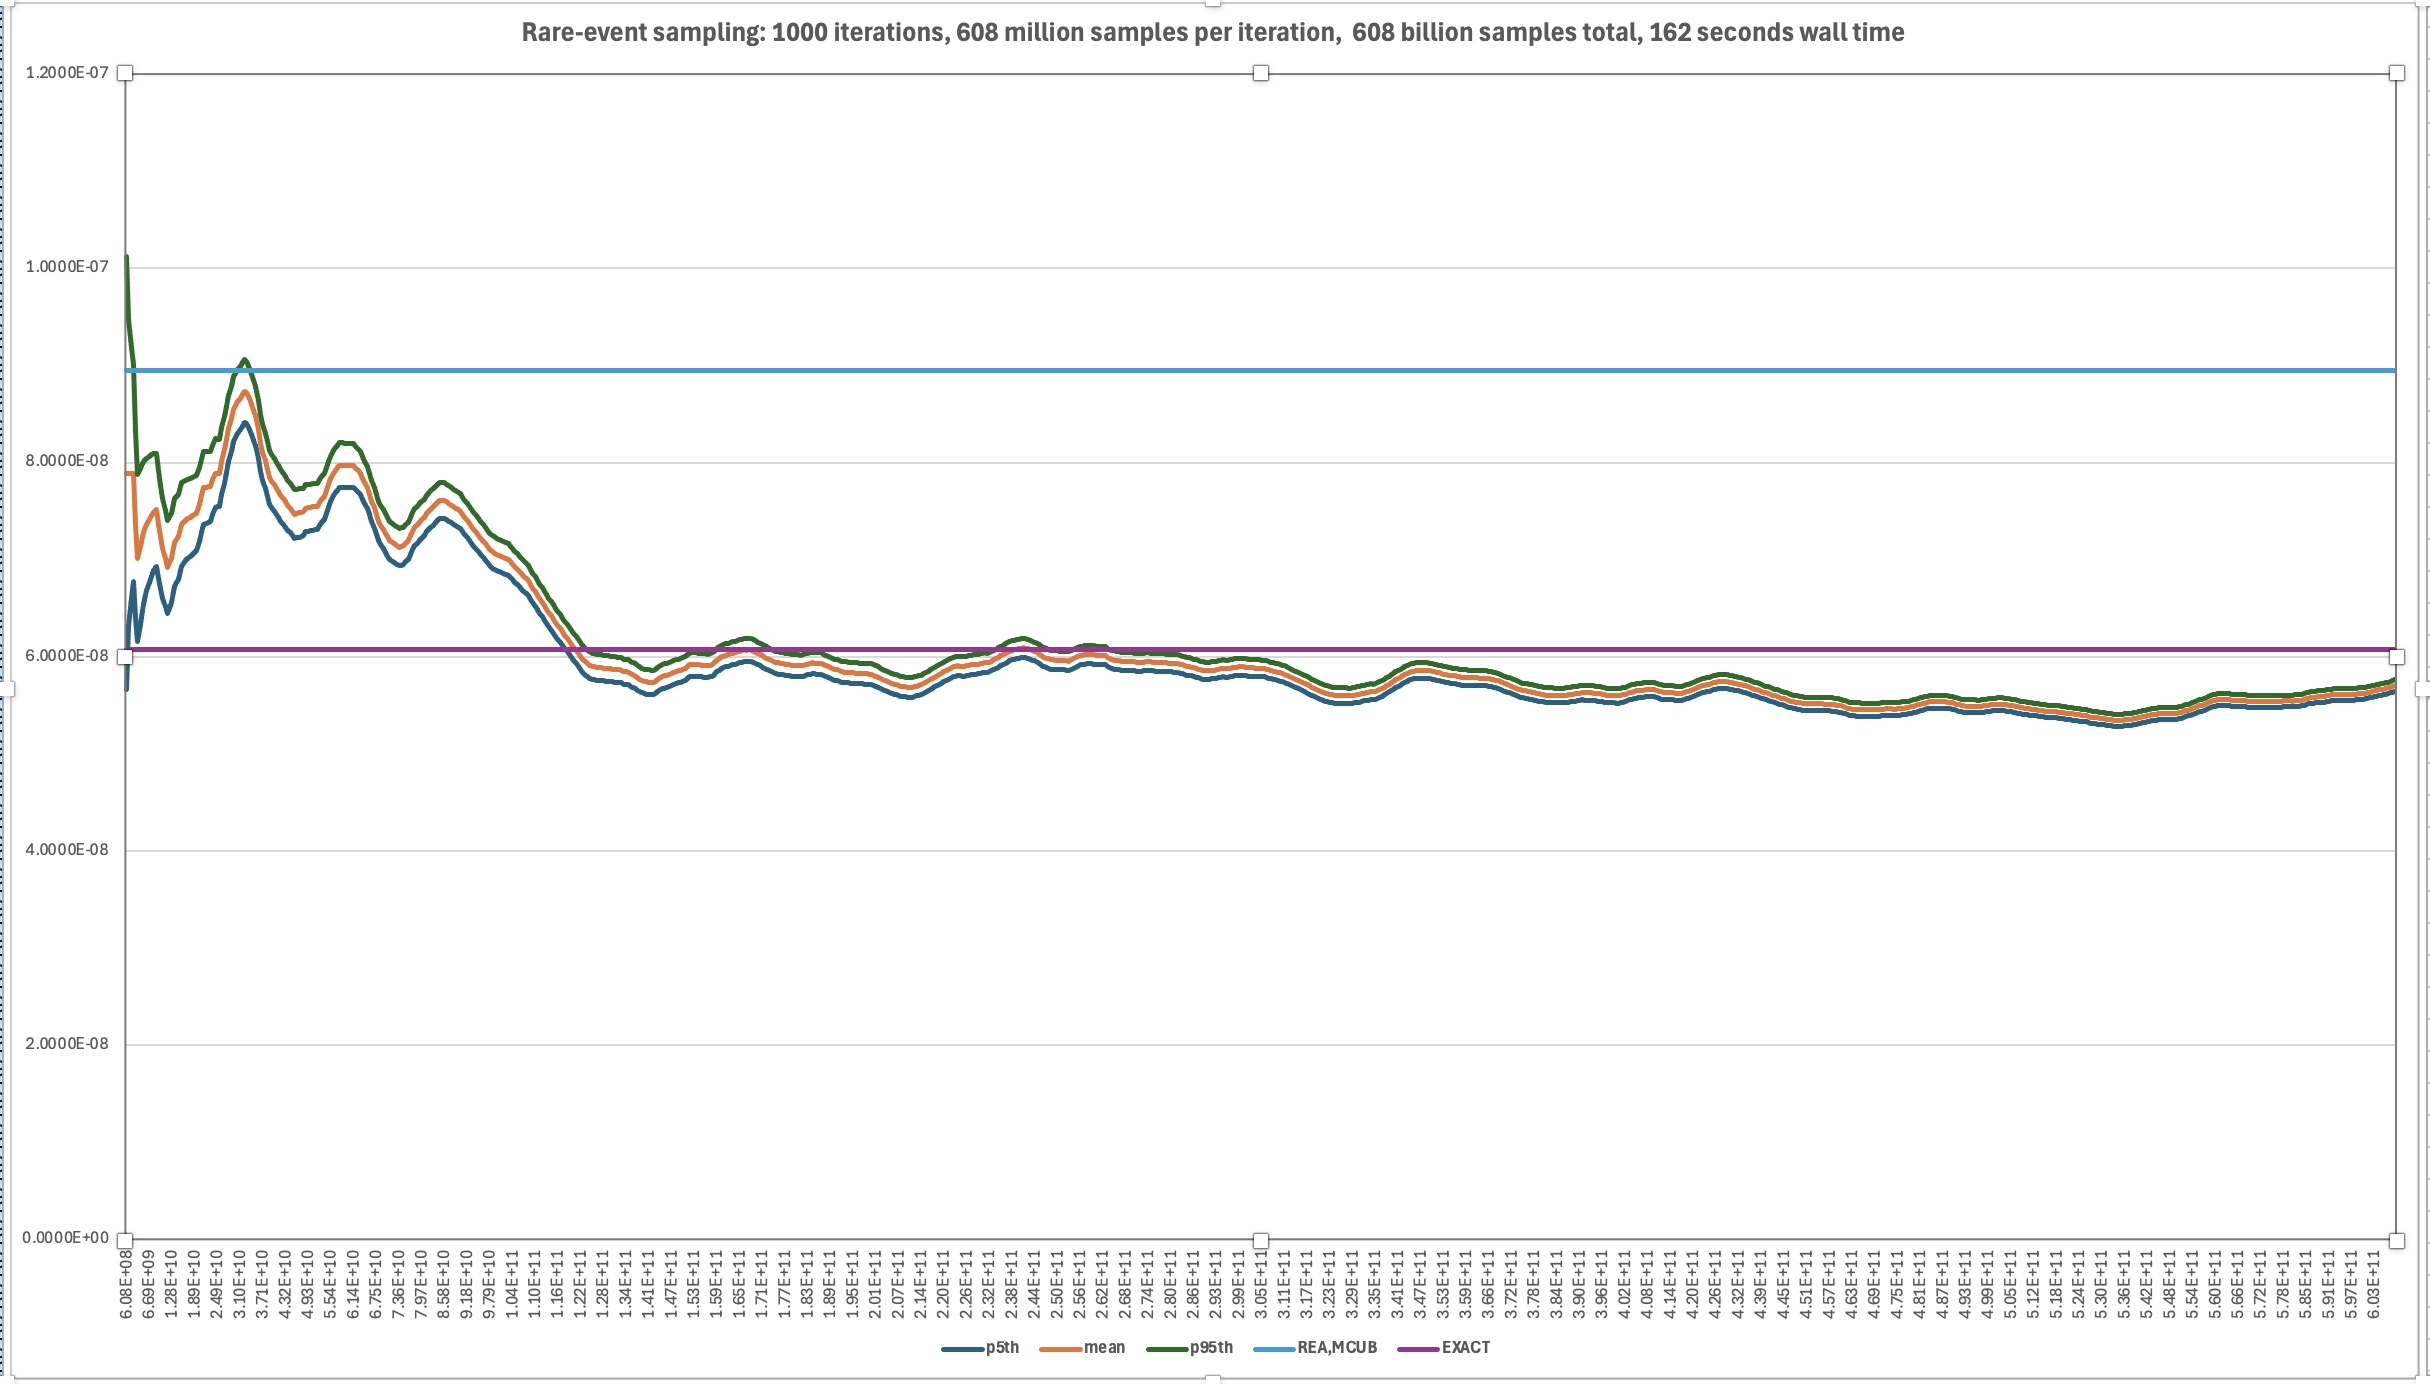
\includegraphics[width=0.7\textwidth]{4_casestudy/rare-event.jpg}
    \label{fig:rare}
\end{figure}
\end{frame}


\subsection{Aralia Fault Tree Data Set - Convergence for Rare Events}
\begin{frame}[allowframebreaks]
    \tiny
\sisetup{table-format=1.2e-2}
\begin{longtable}{@{}llS[table-format=1.2e-2]S[table-format=1.2e-2]S[table-format=1.2e-2]S[table-format=1.2e-2]l@{}}
\label{tab:logp-mae}\\
\toprule
            &          & \multicolumn{3}{c}{\textbf{Mean Absolute Error - log(P)}}       &         &       \\* \cmidrule(lr){3-5}
\multirow{-2}{*}{\textbf{\#}} &
  \multirow{-2}{*}{\textbf{\begin{tabular}[c]{@{}l@{}}Fault\\ Tree\end{tabular}}} &
  \textbf{REA} &
  \textbf{MCUB} &
  \cellcolor[HTML]{F2F2F2}\textbf{Monte Carlo} &
  \multirow{-2}{*}{\textbf{\begin{tabular}[c]{@{}l@{}}MC\\ Samples\end{tabular}}} &
  \multirow{-2}{*}{\textbf{\begin{tabular}[c]{@{}l@{}}Runtime\\ {[}sec{]}\end{tabular}}} \\* \midrule
\endhead
%
\bottomrule
\endfoot
%
\endlastfoot
%
\rowcolor[HTML]{E5E5E5} 
\textbf{1}  & baobab1  & 1.45156E-04 & 1.45156E-04 & 7.61880E-03                         & 2.5E+08 & 0.262 \\
\textbf{2}  & baobab2  & 6.48628E-03 & 6.34705E-03 & \cellcolor[HTML]{F2F2F2}1.54436E-03 & 2.5E+08 & 0.209 \\
\textbf{3}  & baobab3  & 1.21509E-02 & 1.16701E-02 & \cellcolor[HTML]{F2F2F2}2.24843E-04 & 2.4E+08 & 0.259 \\
\textbf{4}  & cea9601  & 9.36195E-02 & 9.32207E-02 & \cellcolor[HTML]{F2F2F2}2.41802E-03 & 1.2E+08 & 0.262 \\
\textbf{5}  & chinese  & 1.08742E-02 & 1.06354E-02 & \cellcolor[HTML]{F2F2F2}2.14601E-03 & 9.4E+08 & 0.277 \\
\textbf{6}  & das9201  & 1.26649E-01 & 1.22765E-01 & \cellcolor[HTML]{F2F2F2}5.49963E-05 & 2.3E+08 & 0.279 \\
\rowcolor[HTML]{E5E5E5} 
\textbf{7}  & das9202  & 7.72743E-05 & 2.57596E-05 & 1.20232E-04                         & 5.2E+08 & 0.295 \\
\textbf{8}  & das9203  & 3.59019E-02 & 3.55935E-02 & \cellcolor[HTML]{F2F2F2}2.31768E-04 & 5.2E+08 & 0.292 \\
\textbf{9}  & das9204  & 1.68086E-01 & 1.68087E-01 & \cellcolor[HTML]{F2F2F2}1.13495E-01 & 6.1E+08 & 0.292 \\
\textbf{10} & das9205  & 9.63825E-02 & 9.63725E-02 & \cellcolor[HTML]{F2F2F2}2.76190E-02 & 3.3E+09 & 0.958 \\
\textbf{11} & das9206  & 5.43561E-02 & 8.89660E-04 & \cellcolor[HTML]{F2F2F2}3.51548E-04 & 2.0E+08 & 0.269 \\
\textbf{12} & das9207  & 1.18486E-01 & 2.45492E-02 & \cellcolor[HTML]{F2F2F2}1.36519E-04 & 9.5E+07 & 0.282 \\
\textbf{13} & das9208  & 4.12808E-02 & 3.81968E-02 & \cellcolor[HTML]{F2F2F2}9.34017E-05 & 2.5E+08 & 0.307 \\
\rowcolor[HTML]{E5E5E5} 
\textbf{14} &
  das9209 &
  2.11242E-02 &
  1.70245E+01 &
   &
  \multicolumn{1}{c}{\cellcolor[HTML]{E5E5E5}-} &
  \multicolumn{1}{c}{\cellcolor[HTML]{E5E5E5}-} \\
\textbf{15} & das9601  & 5.29285E-02 & 5.19122E-02 & \cellcolor[HTML]{F2F2F2}6.67174E-04 & 1.1E+08 & 0.256 \\
\textbf{16} & das9701  & 5.02804E-02 & 3.37565E-02 & \cellcolor[HTML]{F2F2F2}6.22978E-04 & 2.3E+07 & 0.273 \\
\textbf{17} & edf9201  & 1.48012E-01 & 5.36182E-02 & \cellcolor[HTML]{F2F2F2}2.88906E-04 & 1.8E+08 & 0.315 \\
\textbf{18} & edf9202  & 1.07181E-01 & 6.05976E-03 & \cellcolor[HTML]{F2F2F2}4.53900E-04 & 7.8E+07 & 0.271 \\
\textbf{19} & edf9203  & 2.22146E-01 & 1.17293E-01 & \cellcolor[HTML]{F2F2F2}3.27993E-04 & 8.0E+07 & 0.302 \\
\textbf{20} & edf9204  & 2.79531E-01 & 1.05591E-01 & \cellcolor[HTML]{F2F2F2}1.31416E-04 & 8.7E+07 & 0.298 \\
\textbf{21} & edf9205  & 9.94339E-02 & 4.46260E-02 & \cellcolor[HTML]{F2F2F2}5.60146E-05 & 1.9E+08 & 0.284 \\
\rowcolor[HTML]{E5E5E5} 
\textbf{22} & edf9206  & 6.98797E-03 & 7.07775E-03 & -                                   & -       & -     \\
\textbf{23} & edfpa14b & 1.85574E-01 & 9.15983E-02 & \cellcolor[HTML]{F2F2F2}1.04767E-03 & 9.4E+07 & 0.267 \\
\textbf{24} & edfpa14o & 1.86482E-01 & 9.18665E-02 & \cellcolor[HTML]{F2F2F2}3.39049E-04 & 9.8E+07 & 0.275 \\
\textbf{25} & edfpa14p & 3.40010E-02 & 1.66283E-02 & \cellcolor[HTML]{F2F2F2}5.35099E-04 & 2.1E+08 & 0.294 \\
\textbf{26} & edfpa14q & 1.85609E-01 & 9.15366E-02 & \cellcolor[HTML]{F2F2F2}3.33292E-04 & 9.6E+07 & 0.282 \\
\textbf{27} & edfpa14r & 2.48088E-02 & 2.09729E-02 & \cellcolor[HTML]{F2F2F2}9.33865E-04 & 2.1E+08 & 0.294 \\
\textbf{28} & edfpa15b & 2.16329E-01 & 9.37065E-02 & \cellcolor[HTML]{F2F2F2}4.67881E-04 & 1.1E+08 & 0.283 \\
\textbf{29} & edfpa15o & 2.16502E-01 & 9.37627E-02 & \cellcolor[HTML]{F2F2F2}4.06846E-05 & 1.1E+08 & 0.282 \\
\textbf{30} & edfpa15p & 2.52568E-02 & 1.00382E-02 & \cellcolor[HTML]{F2F2F2}3.54344E-04 & 2.6E+08 & 0.299 \\
\textbf{31} & edfpa15q & 2.16329E-01 & 9.37065E-02 & \cellcolor[HTML]{F2F2F2}6.74736E-04 & 1.1E+08 & 0.284 \\
\textbf{32} & edfpa15r & 1.94693E-02 & 1.62668E-02 & \cellcolor[HTML]{F2F2F2}4.04924E-04 & 2.5E+08 & 0.290 \\
\textbf{33} & elf9601  & 1.98107E-02 & 8.08925E-05 & \cellcolor[HTML]{F2F2F2}7.86600E-05 & 2.3E+08 & 0.274 \\
\textbf{34} & ftr10    & 1.22076E-01 & 9.27268E-04 & \cellcolor[HTML]{F2F2F2}1.54844E-04 & 2.1E+08 & 0.297 \\
\textbf{35} & isp9601  & 8.08392E-02 & 6.63074E-02 & \cellcolor[HTML]{F2F2F2}1.13264E-04 & 1.8E+08 & 0.271 \\
\textbf{36} & isp9602  & 1.74572E-02 & 1.47782E-02 & \cellcolor[HTML]{F2F2F2}1.35280E-03 & 2.3E+08 & 0.281 \\
\textbf{37} & isp9603  & 3.82337E-02 & 3.74815E-02 & \cellcolor[HTML]{F2F2F2}3.82344E-03 & 2.7E+08 & 0.278 \\
\textbf{38} & isp9604  & 1.20889E-01 & 8.14313E-02 & \cellcolor[HTML]{F2F2F2}1.88665E-04 & 1.4E+08 & 0.280 \\
\rowcolor[HTML]{E5E5E5} 
\textbf{39} & isp9605  & 6.57344E-03 & 6.57032E-03 & 2.93472E-02                         & 5.0E+08 & 0.262 \\
\textbf{40} & isp9606  & 2.27811E-02 & 1.18983E-02 & \cellcolor[HTML]{F2F2F2}1.30307E-04 & 3.4E+08 & 0.289 \\
\rowcolor[HTML]{E5E5E5} 
\textbf{41} & isp9607  & 2.38880E-02 & 2.38880E-02 & 1.28136E-01                         & 3.8E+08 & 0.282 \\
\textbf{42} & jbd9601  & 1.22001E-01 & 1.35343E-02 & \cellcolor[HTML]{F2F2F2}1.08116E-04 & 5.7E+07 & 0.279 \\
\rowcolor[HTML]{DDDDDD} 
\textbf{43} & nus9601  &            & -           & -                                   & 1.6E+07 & 0.289 \\* \bottomrule
\end{longtable}
\end{frame}


% \begin{frame}{Aralia Fault Tree Dataset}
% show the input dataset table\\
% \end{frame}

% \subsection{Results}
% \begin{frame}{Mar}
% show the input dataset table\\
% \end{frame}
% \section{Research Roadmap}

% %------------------------------------------------
\section{First Section}
%------------------------------------------------

\begin{frame}{Bullet Points}
    \begin{itemize}
        \item Lorem ipsum dolor sit amet, consectetur adipiscing elit 
        \item Aliquam blandit faucibus nisi, sit amet dapibus enim tempus eu
        \item Nulla commodo, erat quis gravida posuere, elit lacus lobortis est, quis porttitor odio mauris at libero
        \item Nam cursus est eget velit posuere pellentesque
        \item Vestibulum faucibus velit a augue condimentum quis convallis nulla gravida
    \end{itemize}
\end{frame}

%------------------------------------------------

\begin{frame}{Blocks of Highlighted Text}
    In this slide, some important text will be \alert{highlighted} because it's important. Please, don't abuse it.

    \begin{block}{Block}
        Sample text
    \end{block}

    \begin{alertblock}{Alertblock}
        Sample text in red box
    \end{alertblock}

    \begin{examples}
        Sample text in green box. The title of the block is ``Examples".
    \end{examples}
\end{frame}

%------------------------------------------------

\begin{frame}{Multiple Columns}
    \begin{columns}[c] % The "c" option specifies centered vertical alignment while the "t" option is used for top vertical alignment

        \column{.45\textwidth} % Left column and width
        \textbf{Heading}
        \begin{enumerate}
            \item Statement
            \item Explanation
            \item Example
        \end{enumerate}

        \column{.45\textwidth} % Right column and width
        Lorem ipsum dolor sit amet, consectetur adipiscing elit. Integer lectus nisl, ultricies in feugiat rutrum, porttitor sit amet augue. Aliquam ut tortor mauris. Sed volutpat ante purus, quis accumsan dolor.

    \end{columns}
\end{frame}

%------------------------------------------------
\section{Second Section}
%------------------------------------------------

\begin{frame}{Table}
    \begin{table}
        \begin{tabular}{l l l}
            \toprule
            \textbf{Treatments} & \textbf{Response 1} & \textbf{Response 2} \\
            \midrule
            Treatment 1         & 0.0003262           & 0.562               \\
            Treatment 2         & 0.0015681           & 0.910               \\
            Treatment 3         & 0.0009271           & 0.296               \\
            \bottomrule
        \end{tabular}
        \caption{Table caption}
    \end{table}
\end{frame}

%------------------------------------------------

\begin{frame}{Theorem}
    \begin{theorem}[Mass--energy equivalence]
        $E = mc^2$
    \end{theorem}
\end{frame}

%------------------------------------------------

\begin{frame}{Figure}
    Uncomment the code on this slide to include your own image from the same directory as the template .TeX file.
    %\begin{figure}
    %\includegraphics[width=0.8\linewidth]{test}
    %\end{figure}
\end{frame}

%------------------------------------------------

\begin{frame}[fragile] % Need to use the fragile option when verbatim is used in the slide
    \frametitle{Citation}
    An example of the \verb|\cite| command to cite within the presentation:\\~
    This statement requires citation \cite{earthperson_combined_2023}.
\end{frame}

%------------------------------------------------

% \begin{frame}{References}
%     \footnotesize
%     \bibliography{reference.bib}
%     \bibliographystyle{apalike}
% \end{frame}

%------------------------------------------------

\begin{frame}
    \Huge{\centerline{\textbf{The End}}}
\end{frame}

%----------------------------------------------------------------------------------------

\end{document}